\section{Introduction}
Structural complexity of RNA molecules is vast and so are their modes of interaction with proteins \citep{jones2001protein}. Although there has been an ever-expanding repertoire of structural data on the PDB, there is a lack of data resources which systematically analyze these interactions. In addition, recent advances in artificial intelligence have made high throughput prediction of protein-RNA complex structures viable \citep{Abramson2024, watson2023novo}. RNAproDB is a webserver where a user can upload a protein-RNA complex and explore analyzed results covering a multitude of aspects (e.g., direct and water-mediated hydrogen bonds, base-pairing annotations, nucleotide modifications, secondary structural features). Compared to existing resources, which often focus on the RNA structure alone and provide a particular way of visualization \citep{Kerpedjiev2015, Yang2003}, or use a representation which is very coarse-grained \citep{chojnowski2014rna}, RNAproDB provides three different algorithms for visualizing the RNA topology along with the interacting protein residues: a new design based on partial projection of the structure (RNA and interacting protein residues), tertiary structure aware mapping \citep{Mitra2024rnascape}, secondary structure-based mapping \citep{Kerpedjiev2015}. This information is presented via a highly interactive interface explorer combined with sequence and 3D-structure viewers, and a secondary structure selector. Tabular data is also available. Another novel functionality, subgraph exploration, allows a user to explore parts of the structure (e.g., a particular junction region) via the interface explorer. Subgraph selections can be manually entered or automatically selected from the secondary structure selector. As of our knowledge, no existing tool offers such capability. In addition to the webserver, we offer pre-analyzed structures containing RNA, from the PDB, in the form of a searchable collection. With a cutoff of 10,000 monomers per biological assembly and molecular weight cut off of 800 kDa on the asymmetric unit, the initial collection of RNAproDB provides around 3,500 biological assemblies containing RNA molecules. RNAproDB will be automatically updated weekly with new PDB entries. We believe RNAproDB will be a valuable resource for the scientific community interested in RNA biology, protein-nucleic acid interaction and function, structure prediction, and drug design.

\begin{center}
    \begin{figure}
    \makebox[\textwidth]{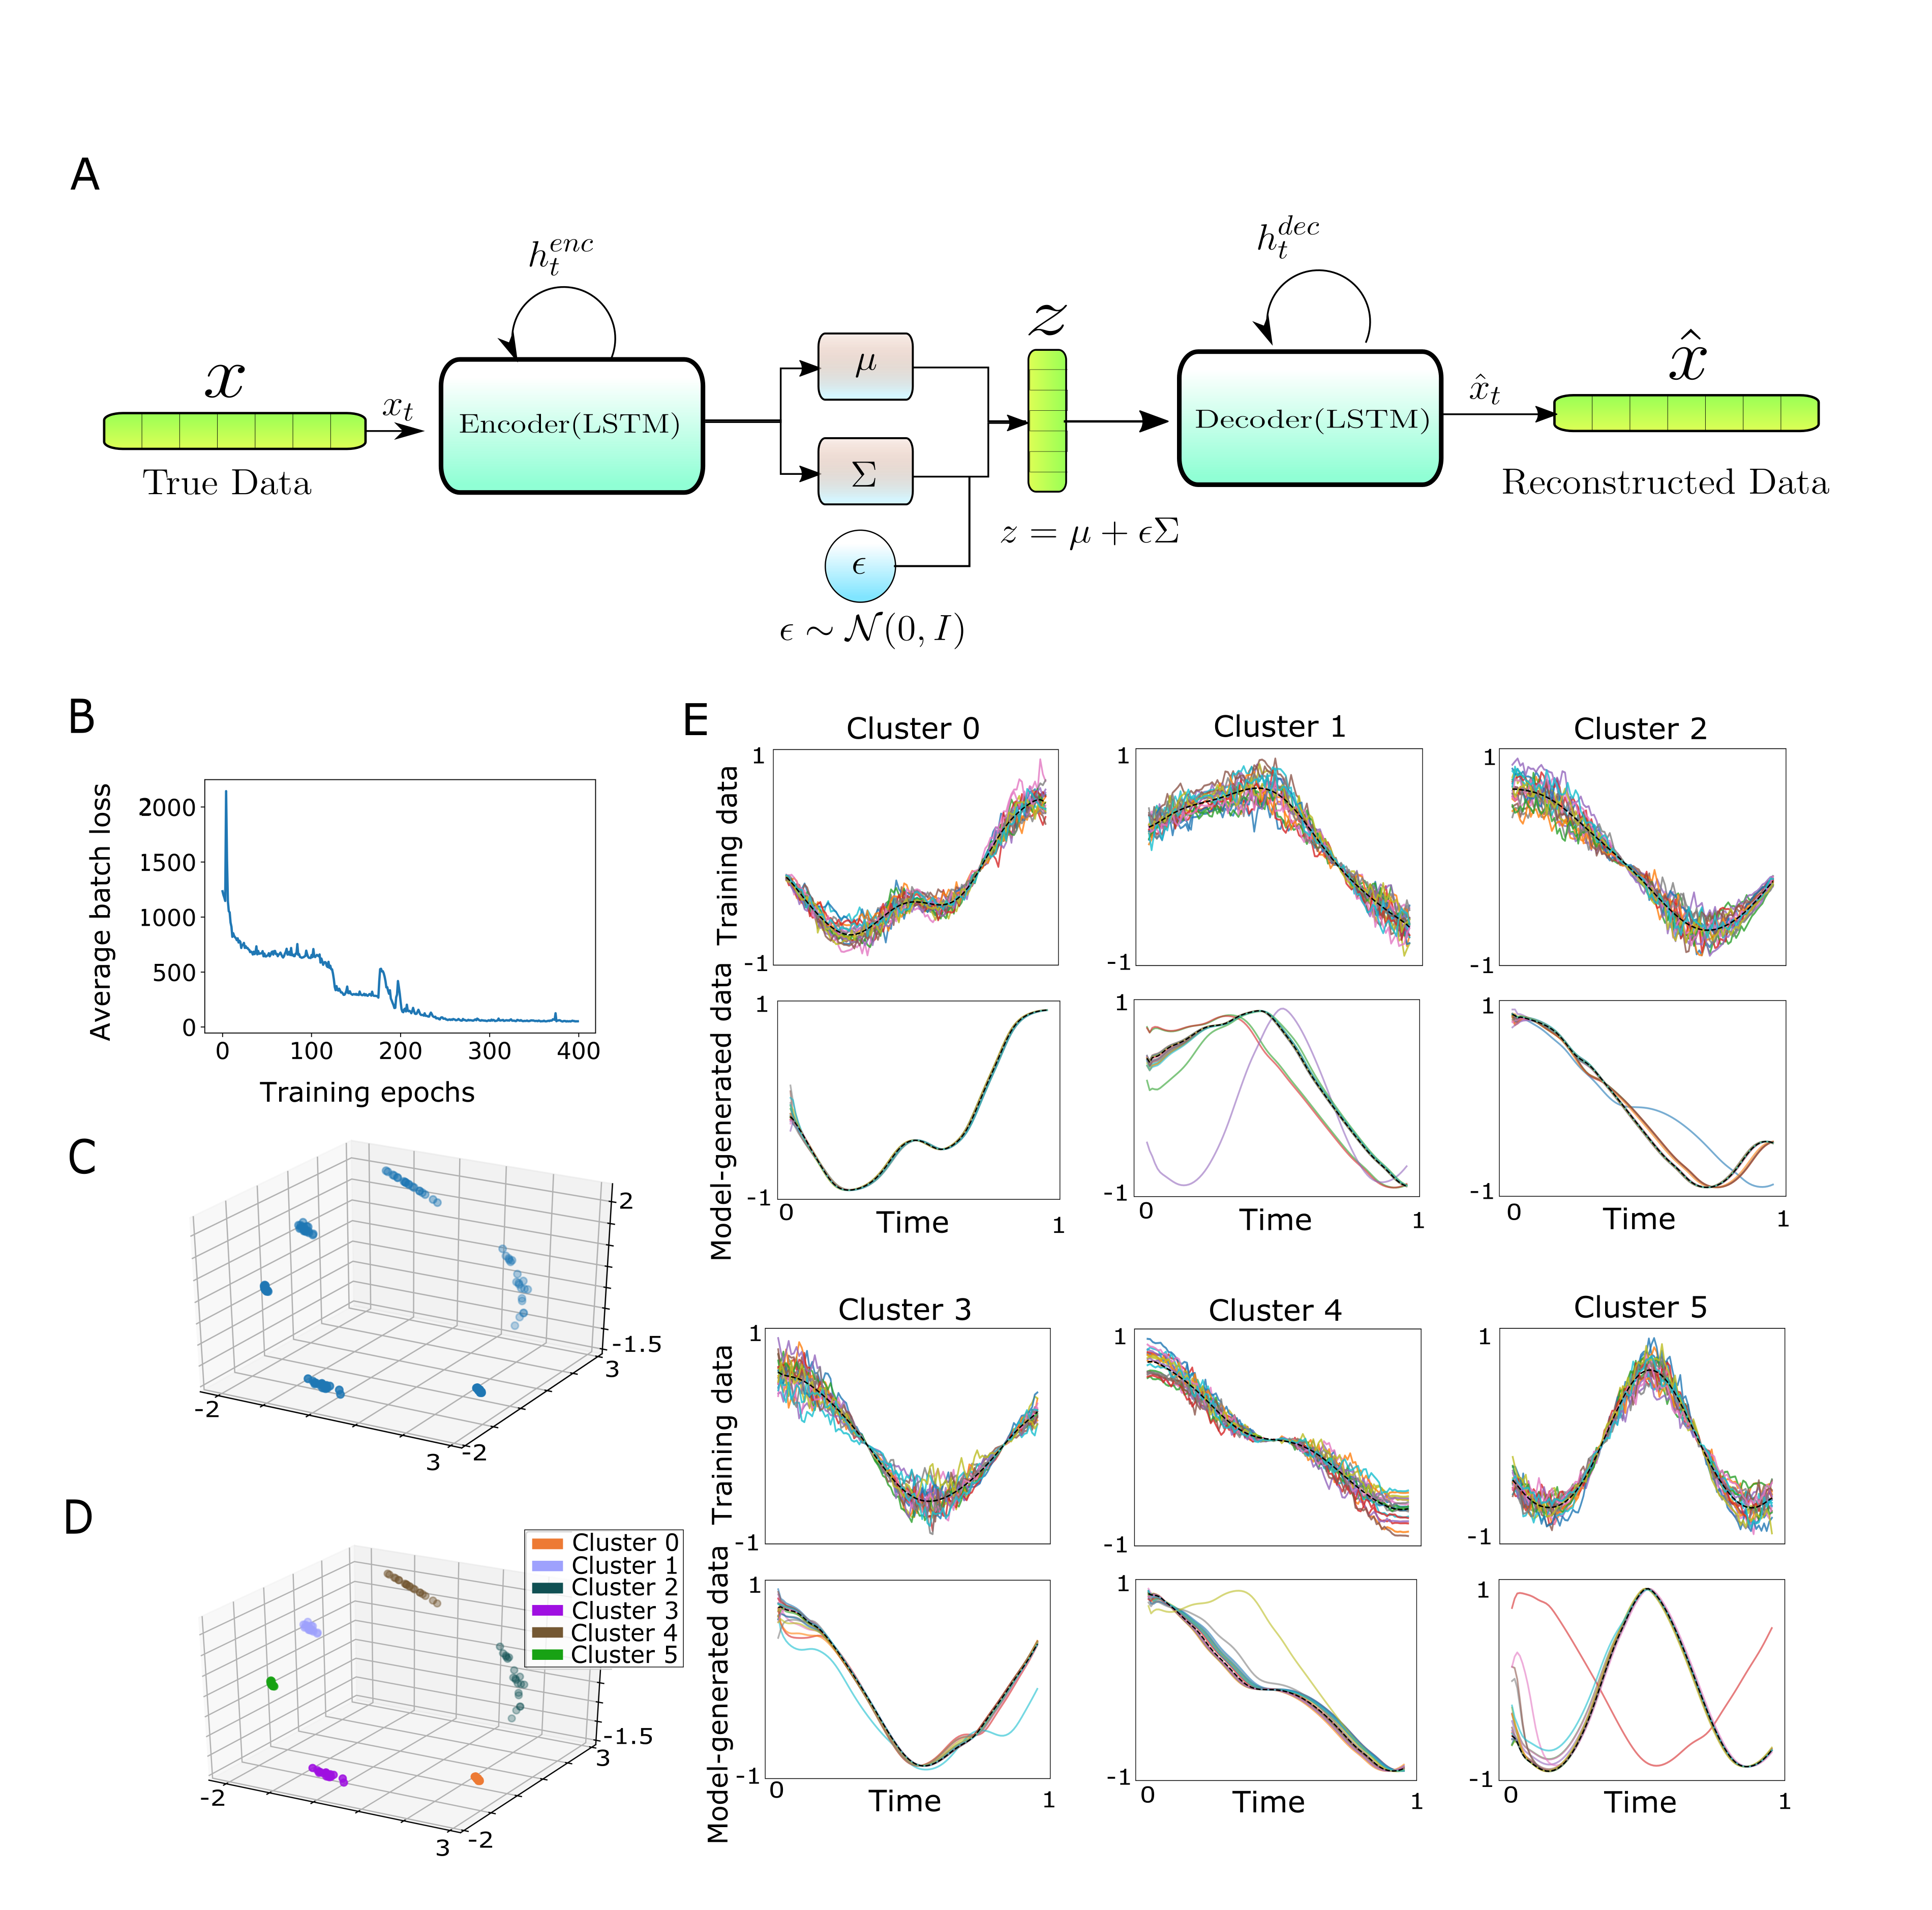
\includegraphics[width=0.8\paperwidth]{./rnaprodbfigs/fig1.png}}
 % archetecture.png: 1149x508 px, 72dpi, 40.53x17.92 cm, bb=0 0 1149 508
        \caption[Key aspects of this update to DNAproDB.]{\textbf{Key aspects of this update to DNAproDB.} ({\bf A}) Automatic update and separated external annotation incorporation scheme.  ({\bf B})  Different nucleic acid layout options in with added tertiary structure aware RNAscape layout, shown for PDB ID: 3LDY. ({\bf C}) Water-mediated hydrogen bond annotation. ({\bf D}) Various improvements in other aspects of DNAproDB. }
  \label{fig:rnaprodb1}
\end{figure}
\end{center}

\section{Interface explorer}

The 'Interface explorer' for RNAproDB is freshly designed to present an interaction graph of the RNA structure along with interacting protein residues. The explorer present three different layout algorithm options, selectable by the user. two of these options are secondary structure based (computed using ViennaRNA \citep{Lorenz2011}) and tertiary structure aware mapping based (computed using RNAscape \citep{Mitra2024rnascape}). The third (default) option is a new mapping scheme produced by prjecting the RNA residues and only interacting protein residues into the 2D plane maximizing their spatial variance \citep{Pearson1901}. We call this method ``Partial projection" (instead of the whole structure, it only projects the RNA and interacting protein components). In our observation, this scheme is visually intuitive for exploring corresponding 3D structure. The user is free to choose between the three layouts. In each case, the protein residues are placed using a force directed layout scheme \citep{bostock2012fl}. We demonstrate the three layout schemes for a valyl-tRNA synthetase-tRNA complex (PDB ID: 1IVS) (\blue{Fig. \ref{fig:rnaprodb1}A}). The partial projection-based layout is shown in \blue{Fig. \ref{fig:rnaprodb1}B}. This layout reflects the helical turns, making the best coreespondance with the 3D structure. The RNAscape \citep{Mitra2024rnascape} layout (\blue{Fig. \ref{fig:rnaprodb1}C}) is cleaner and more suitable for users used to ladder-like representation.  The secondary structure based layout, shown in \blue{Fig. \ref{fig:rnaprodb1}D}, although familiar, suffers from tertiary interactions within RNA and protein-RNA interactions criss-crossing the view. 

\section{Secondary structure selector and subgraph exploration}

A more coarse grained diagram is also computed as part of the processing piepline for RNAproDB. This diagram reflects the different secondary structure elements as one node each, interaction edges corresponding to residues involved in one secondary structure element with another are collapsed into one edge. This view is presented to serve as a selectable by the user, named "Secondary structure selector". An example is shown for PDB ID: 1UN6 \blue{Fig. \ref{fig:rnaprodb2}D}). The corresponding Secondary structure selector is shown in \blue{Fig. \ref{fig:rnaprodb2}E}. The partial projection-based layout for this structure is presented in \blue{Fig. \ref{fig:rnaprodb2}F}. 

Whenever a user clicks a particular node (e.g. `Stem 3' in \blue{Fig. \ref{fig:rnaprodb2}E}), corresponding nucleic acid residue ids are populated into the subgraph generation dialogue. The user can now click the "Generate subgraph" button to generate and explore the subgraph (upto first order neighbors) via the interface explorer (\blue{Fig. \ref{fig:rnaprodb2}G}). Beyond clicking the secondary structure selector, a subgraph selection can also be manually entered or selected from the Sequence viewer or Interface explorer. 

\begin{center}
    \begin{figure}
    \makebox[\textwidth]{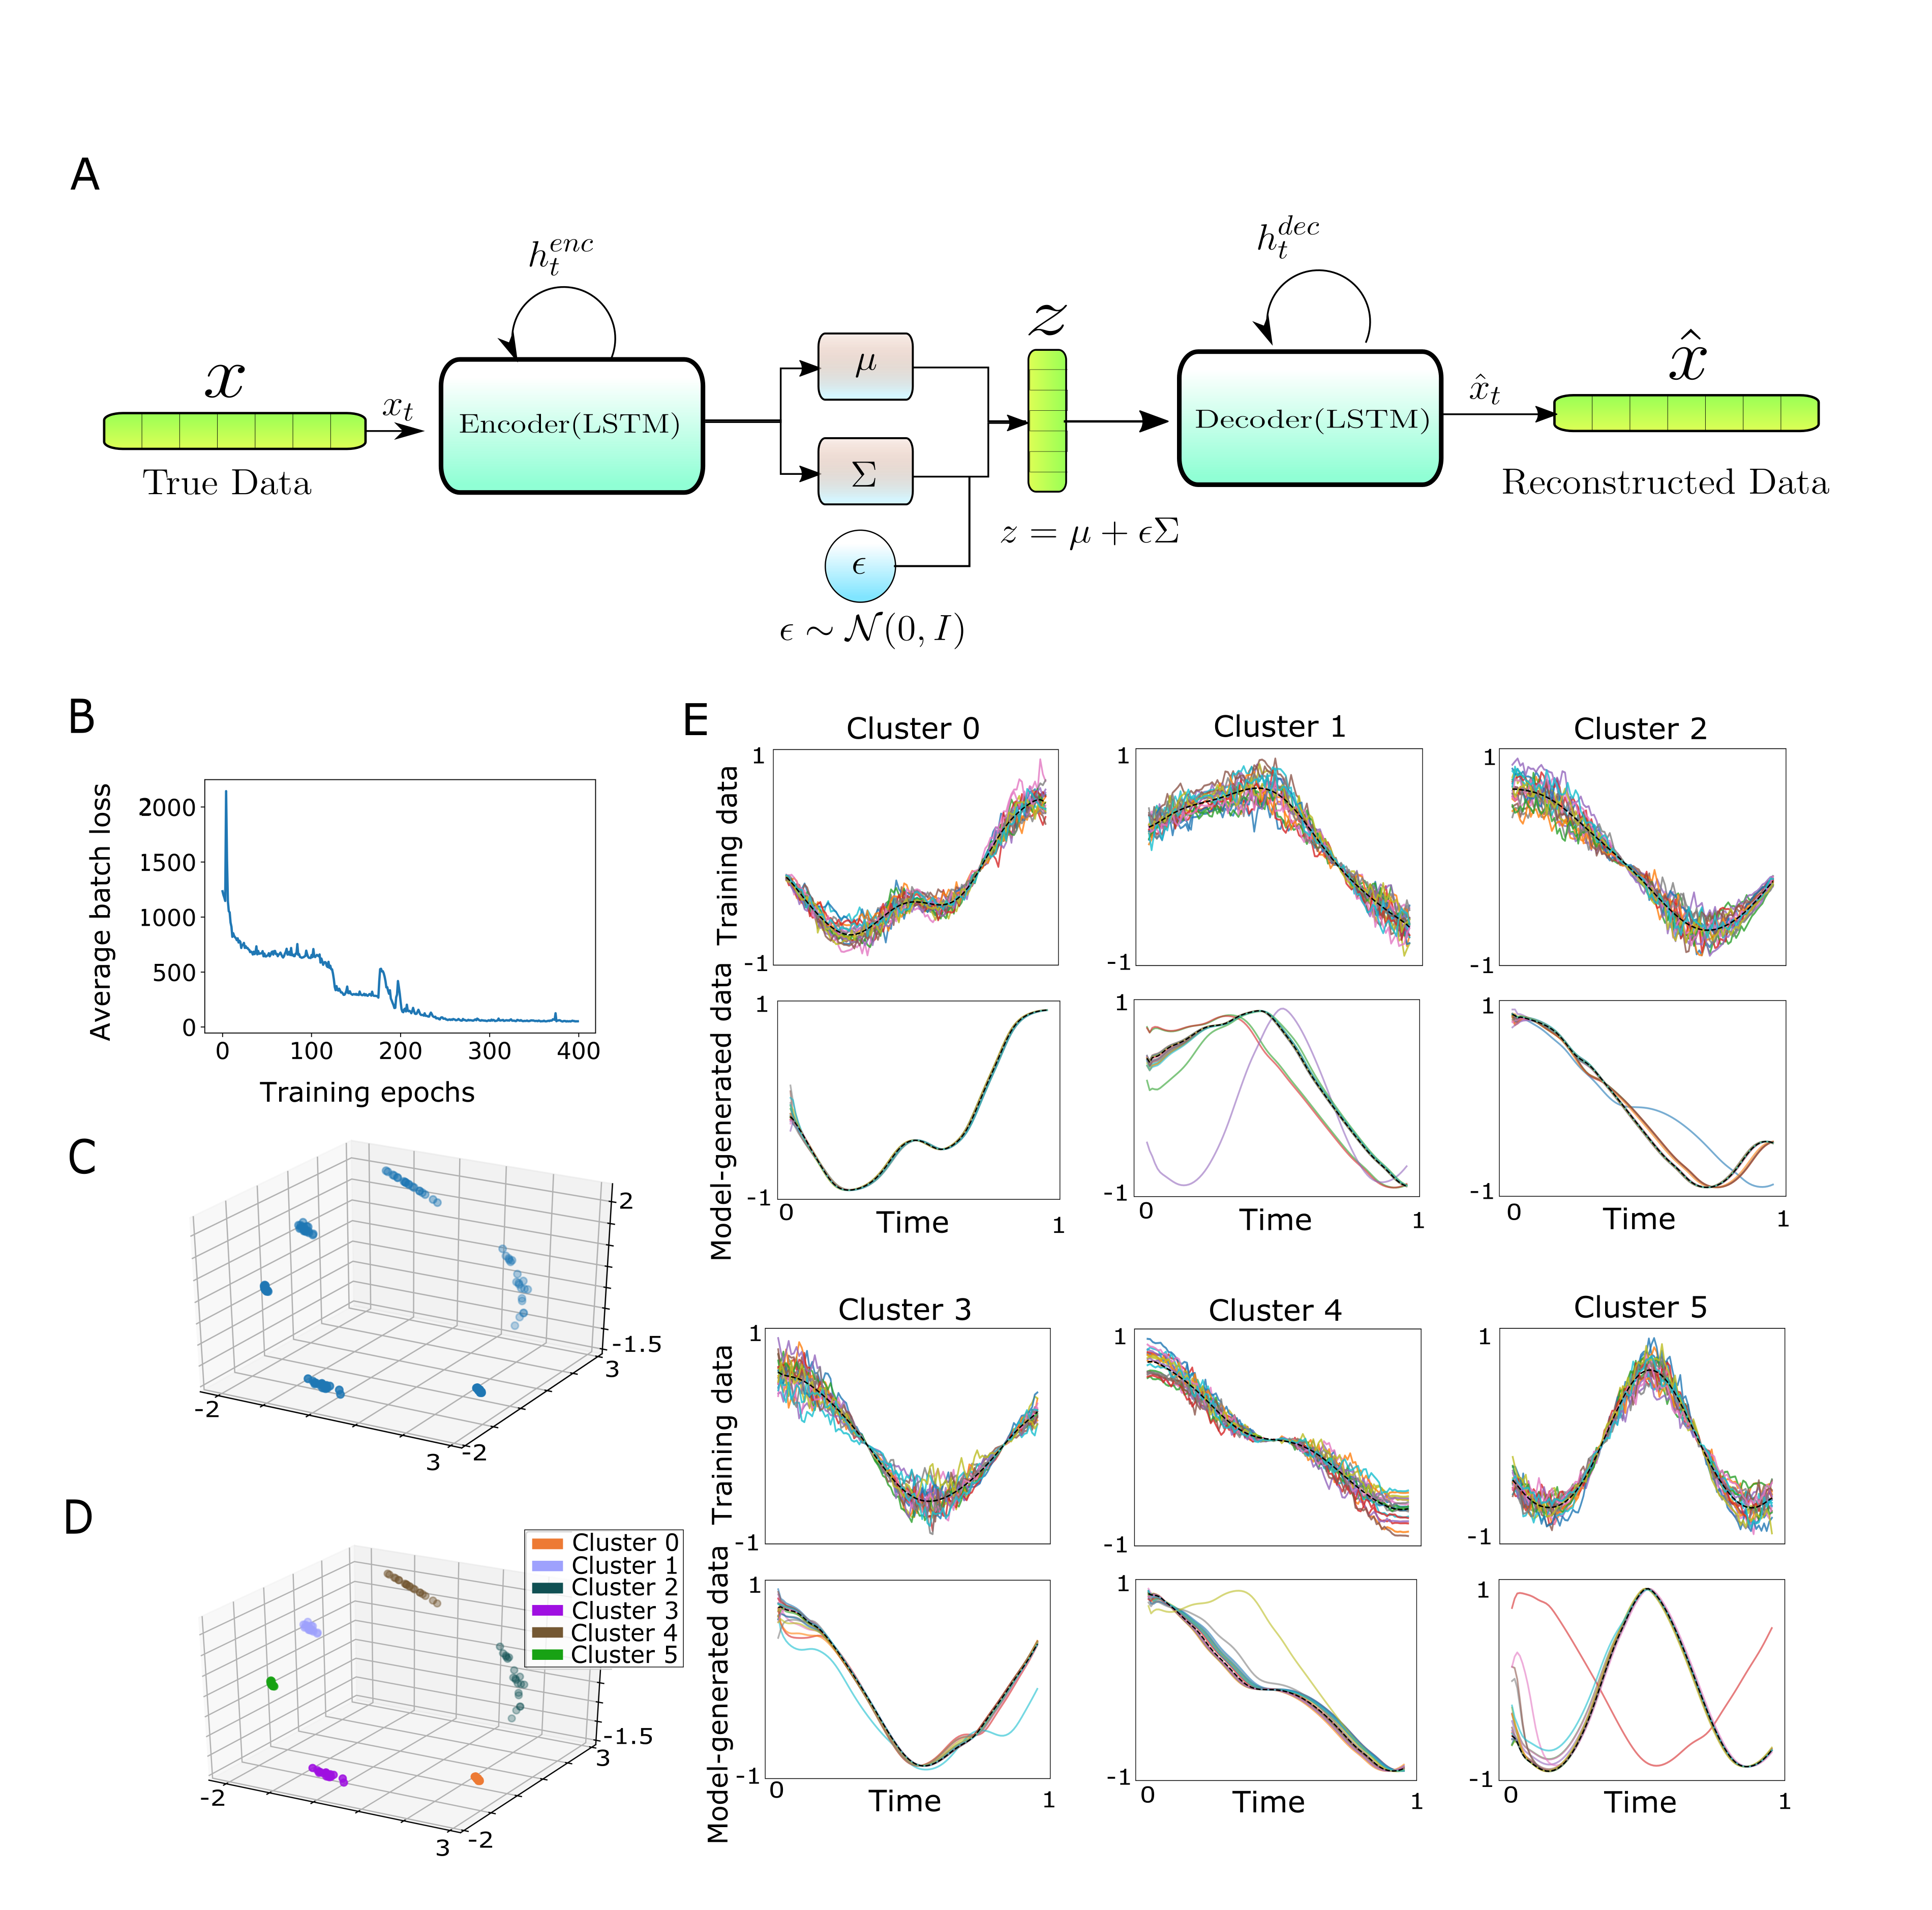
\includegraphics[width=0.8\paperwidth]{./rnaprodbfigs/fig2.png}}
 % archetecture.png: 1149x508 px, 72dpi, 40.53x17.92 cm, bb=0 0 1149 508
        \caption[Key aspects of this update to DNAproDB.]{\textbf{Key aspects of this update to DNAproDB.} ({\bf A}) Automatic update and separated external annotation incorporation scheme.  ({\bf B})  Different nucleic acid layout options in with added tertiary structure aware RNAscape layout, shown for PDB ID: 3LDY. ({\bf C}) Water-mediated hydrogen bond annotation. ({\bf D}) Various improvements in other aspects of DNAproDB. }
  \label{fig:rnaprodb2}
\end{figure}
\end{center}

\section{RNA-RNA water mediated interactions}

\begin{center}
    \begin{figure}
    \makebox[\textwidth]{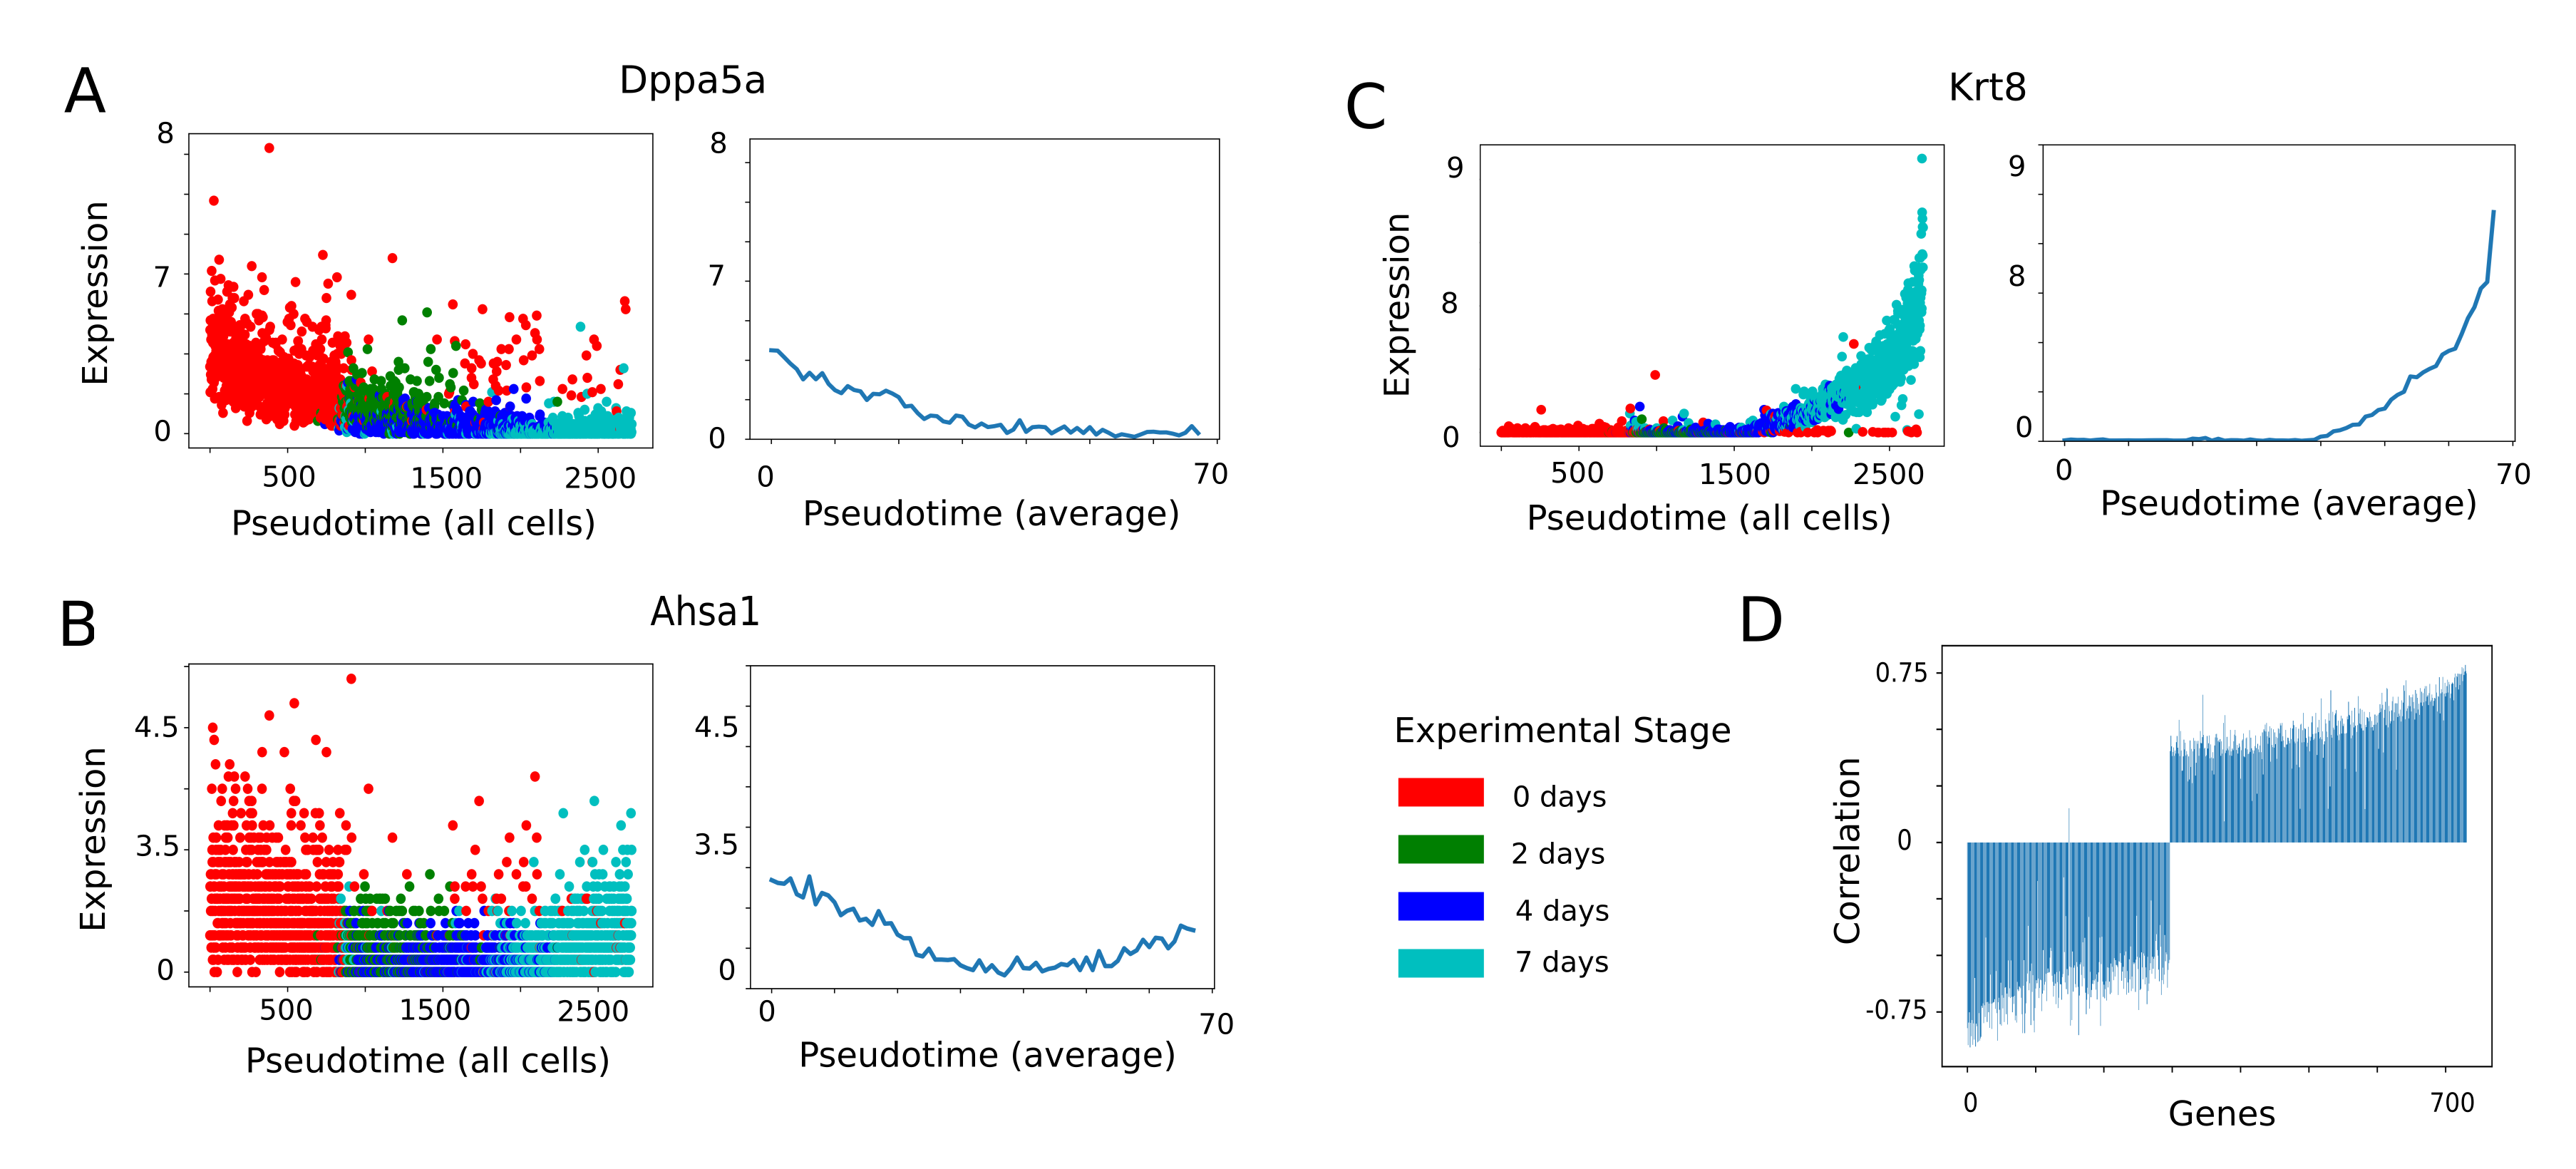
\includegraphics[width=0.8\paperwidth]{./rnaprodbfigs/fig3.png}}
 % archetecture.png: 1149x508 px, 72dpi, 40.53x17.92 cm, bb=0 0 1149 508
        \caption[Key aspects of this update to DNAproDB.]{\textbf{Key aspects of this update to DNAproDB.} ({\bf A}) Automatic update and separated external annotation incorporation scheme.  ({\bf B})  Different nucleic acid layout options in with added tertiary structure aware RNAscape layout, shown for PDB ID: 3LDY. ({\bf C}) Water-mediated hydrogen bond annotation. ({\bf D}) Various improvements in other aspects of DNAproDB. }
  \label{fig:rnaprodb3}
\end{figure}
\end{center}